%
% $RCSfile: self_awareness.tex,v $
%
% Copyright (C) 2002-2008. Christian Heller.
%
% Permission is granted to copy, distribute and/or modify this document
% under the terms of the GNU Free Documentation License, Version 1.1 or
% any later version published by the Free Software Foundation; with no
% Invariant Sections, with no Front-Cover Texts and with no Back-Cover
% Texts. A copy of the license is included in the section entitled
% "GNU Free Documentation License".
%
% http://www.cybop.net
% - Cybernetics Oriented Programming -
%
% http://www.resmedicinae.org
% - Information in Medicine -
%
% Version: $Revision: 1.1 $ $Date: 2008-08-19 20:41:08 $ $Author: christian $
% Authors: Christian Heller <christian.heller@tuxtax.de>
%

\subsection{Self Awareness}
\label{self_awareness_heading}
\index{Self Awareness}
\index{Mind}
\index{Brain}
\index{Vegetative Nerve System}
\index{Animalic Nerve System}
\index{Agent}
\index{Agent Oriented Programming}
\index{AGOP}
\index{Capabilities of an Agent}
\index{Mental State of an Agent}

One of the particular characteristics of human beings is their ability for
\emph{Self Awareness}. It contrasts the human- with an animal mind because it
permits humans not only to understand what is going on in their environment,
but also themselves and their being in this world. In other words, the
\emph{Mind} knows about itself and about its existence in form of the human
organ called \emph{Brain}, as its physical carrier and as the place of
thinking.

Of course, the mind also knows about further organs and body parts. Some of the
concepts stored in it contain the characteristics of a human being. This
knowledge of the structure of the human body is necessary for the mind to be
able to steer it. While the functions for living are \emph{passively}
controlled by the \emph{vegetative} (unconscious) nerve system, sensoric and
motoric (input/ output) organs need to be controlled \emph{actively}, by the
\emph{animalic} (conscious) nerve system.

A system also needs to know about its own abilities, in order to be able to
communicate. It has to have a concept of its communication organs/ devices,
spoken languages etc. This counts for a human- as for a computer system. The
\emph{Agent} systems used in \emph{Agent Oriented Programming} (AGOP) (section
\ref{agent_oriented_programming_heading}) know about their \emph{Capabilities},
which are stored together with other knowledge as their \emph{Mental State}.

%
% $RCSfile: human_body.tex,v $
%
% Copyright (C) 2002-2008. Christian Heller.
%
% Permission is granted to copy, distribute and/or modify this document
% under the terms of the GNU Free Documentation License, Version 1.1 or
% any later version published by the Free Software Foundation; with no
% Invariant Sections, with no Front-Cover Texts and with no Back-Cover
% Texts. A copy of the license is included in the section entitled
% "GNU Free Documentation License".
%
% http://www.cybop.net
% - Cybernetics Oriented Programming -
%
% http://www.resmedicinae.org
% - Information in Medicine -
%
% Version: $Revision: 1.1 $ $Date: 2008-08-19 20:41:07 $ $Author: christian $
% Authors: Christian Heller <christian.heller@tuxtax.de>
%

\subsubsection{Human Body}
\label{human_body_heading}
\index{Human Body}
\index{Sensoric Organs}
\index{Motoric Organs}
\index{Human Senses}
\index{Nerve Cell}
\index{Muscle Cell}
\index{Information Reception}
\index{Information Sending}

Figure \ref{human_figure} shows parts of the animalic nerve system of a human
being. \emph{Sensoric} organs are used for information input; \emph{motoric}
organs for information output.

\begin{figure}[ht]
    \begin{center}
        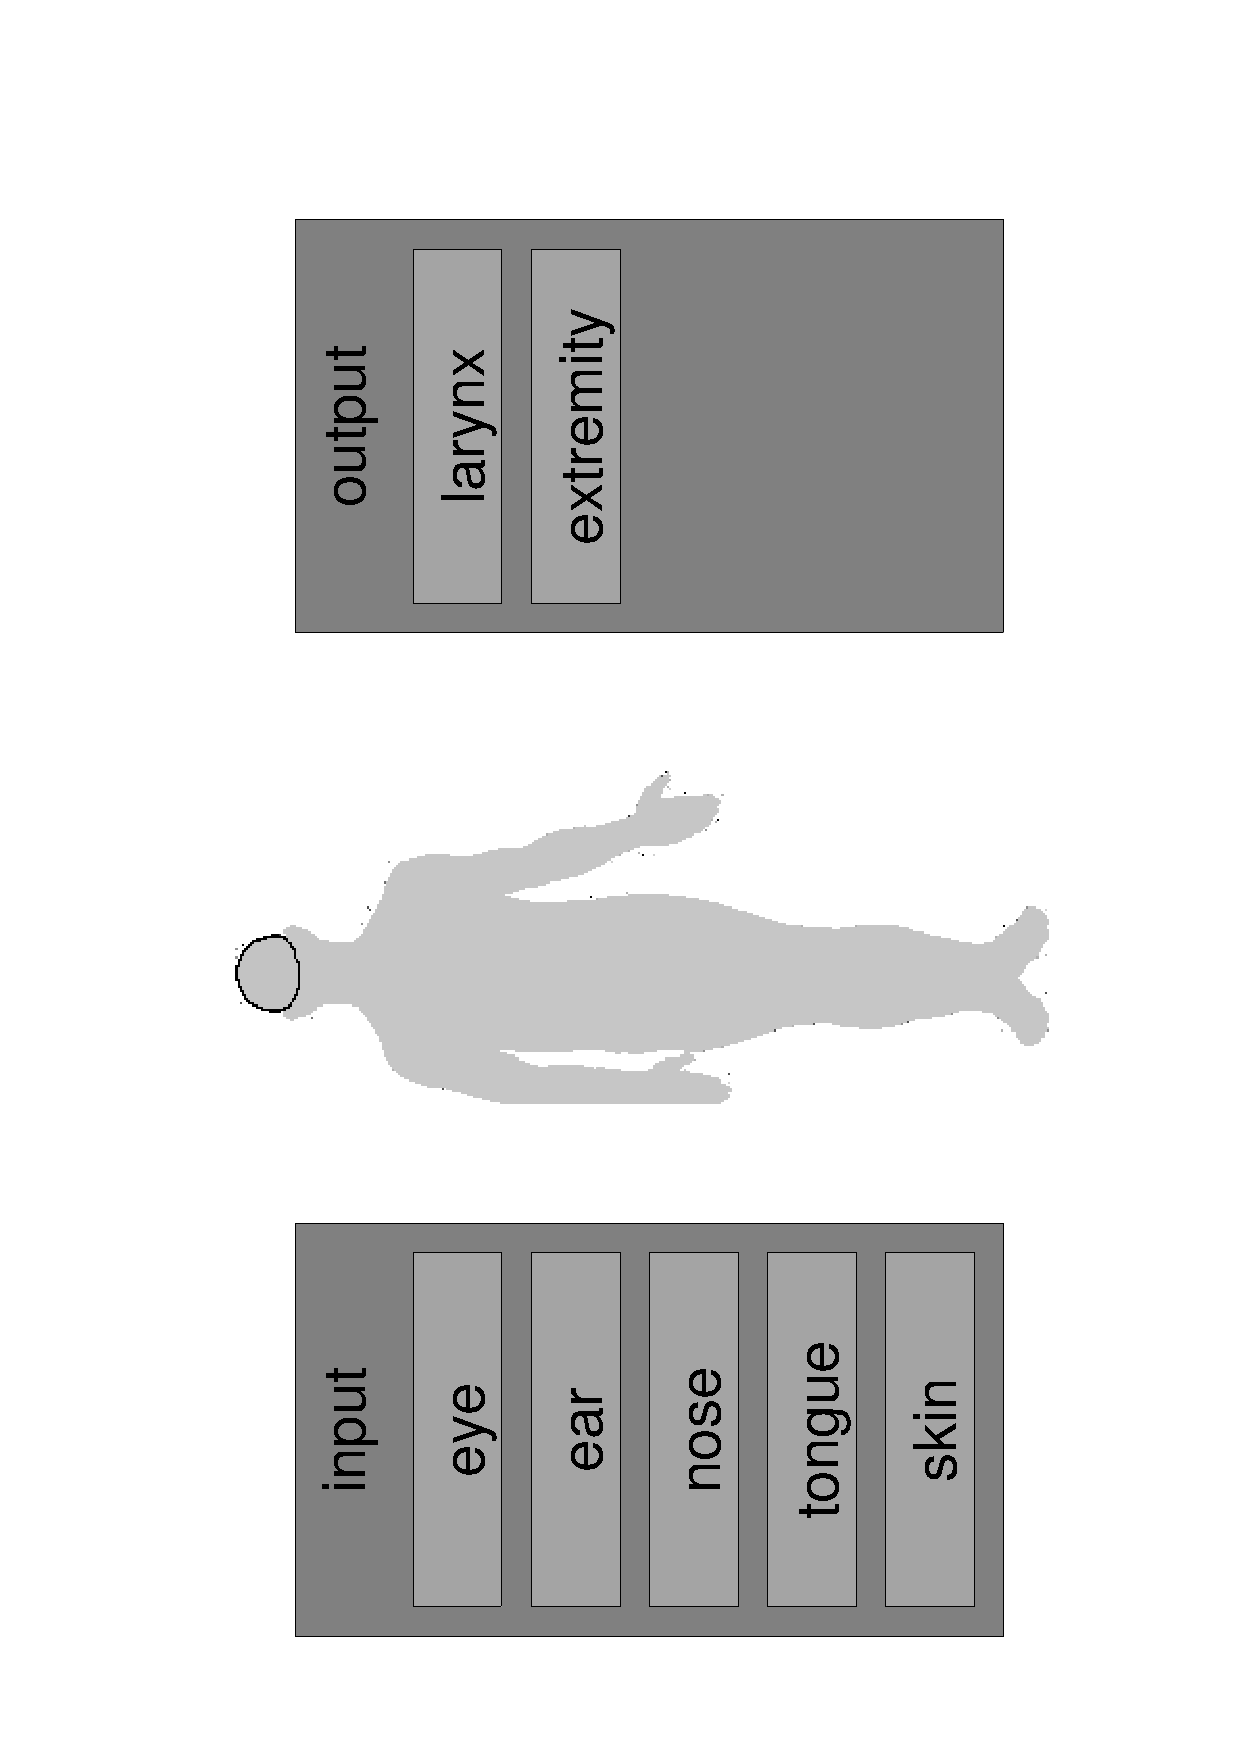
\includegraphics[scale=0.3,angle=-90]{graphic/human.pdf}
        \caption{Human Body with Sensoric and Motoric Organs}
        \label{human_figure}
    \end{center}
\end{figure}

The five (seven) human senses were already shown in table \ref{senses_table}.
They are able to receive signals which are transported by different mediums.
The transport mechanisms rely on various physical and chemical \emph{Effects},
as shown in table \ref{effects_table}. Each sense is represented by an
\emph{Organ}. The optic cells of the retina of an \emph{Eye} bundle light
stimuli which the optic nerve forwards as electrical signal to the brain. The
inner \emph{Ear} transforms oscillation frequencies of sound-waves into
electrical signals to send on to the brain. And so forth.

\begin{table}[ht]
    \begin{center}
        \begin{footnotesize}
        \begin{tabular}{| p{30mm} | p{50mm} | p{25mm} |}
            \hline
            \textbf{Effect} & \textbf{Science} & \textbf{Sense}\\
            \hline
            Oscillation, Wave & Physics, Mechanics & Seeing, Hearing\\
            \hline
            Density, Temperature & Physics, Mechanics, Thermodynamics & Tactile\\
            \hline
            Aroma & Chemistry & Smelling, Tasting\\
            \hline
        \end{tabular}
        \end{footnotesize}
        \caption{Effects as Basis of Sensing}
        \label{effects_table}
    \end{center}
\end{table}

While the \emph{Reception} of information is based on \emph{Nerve Cells}, it is
\emph{Muscle Cells} which are responsible for information \emph{Sending}.
Humans communicate for example through visual \emph{Gestures} using their
\emph{Extremities} or through acoustical \emph{Talking} using their
\emph{Larynx}/ \emph{Vocal Chords}. The latter, too, is based on muscle
activity.

%
% $RCSfile: computer_hardware.tex,v $
%
% Copyright (C) 2002-2008. Christian Heller.
%
% Permission is granted to copy, distribute and/or modify this document
% under the terms of the GNU Free Documentation License, Version 1.1 or
% any later version published by the Free Software Foundation; with no
% Invariant Sections, with no Front-Cover Texts and with no Back-Cover
% Texts. A copy of the license is included in the section entitled
% "GNU Free Documentation License".
%
% http://www.cybop.net
% - Cybernetics Oriented Programming -
%
% http://www.resmedicinae.org
% - Information in Medicine -
%
% Version: $Revision: 1.1 $ $Date: 2008-08-19 20:41:06 $ $Author: christian $
% Authors: Christian Heller <christian.heller@tuxtax.de>
%

\subsubsection{Computer Hardware}
\label{computer_hardware_heading}
\index{Computer Hardware}
\index{Human Being}
\index{Technical Environment}
\index{Biological Environment}

Gilbert Carl Herschberger II writes \cite{josgeneral}: \textit{A computer is a
grossly oversimplified model of a human being. Humans can learn more about
themselves by working with this model. And, they might learn more about what
makes a good model by looking at themselves.} To the many analogies a computer
has with a human being belong its input/ output (i/o) devices (figure
\ref{computer_figure}), many of which have an equivalent organ in the human
body:

\begin{itemize}
    \item[-] \emph{Eye}: Camera, Scanner
    \item[-] \emph{Ear}: Microphone
    \item[-] \emph{Nose, Tongue}: Sensors
    \item[-] \emph{Skin}: Keyboard, Mouse, Joystick
    \item[-] \emph{Larynx}: Loudspeaker
    \item[-] \emph{Extremity}: Monitor, Printer, Braille Panel, Arm, Wheel
\end{itemize}

\begin{figure}[ht]
    \begin{center}
        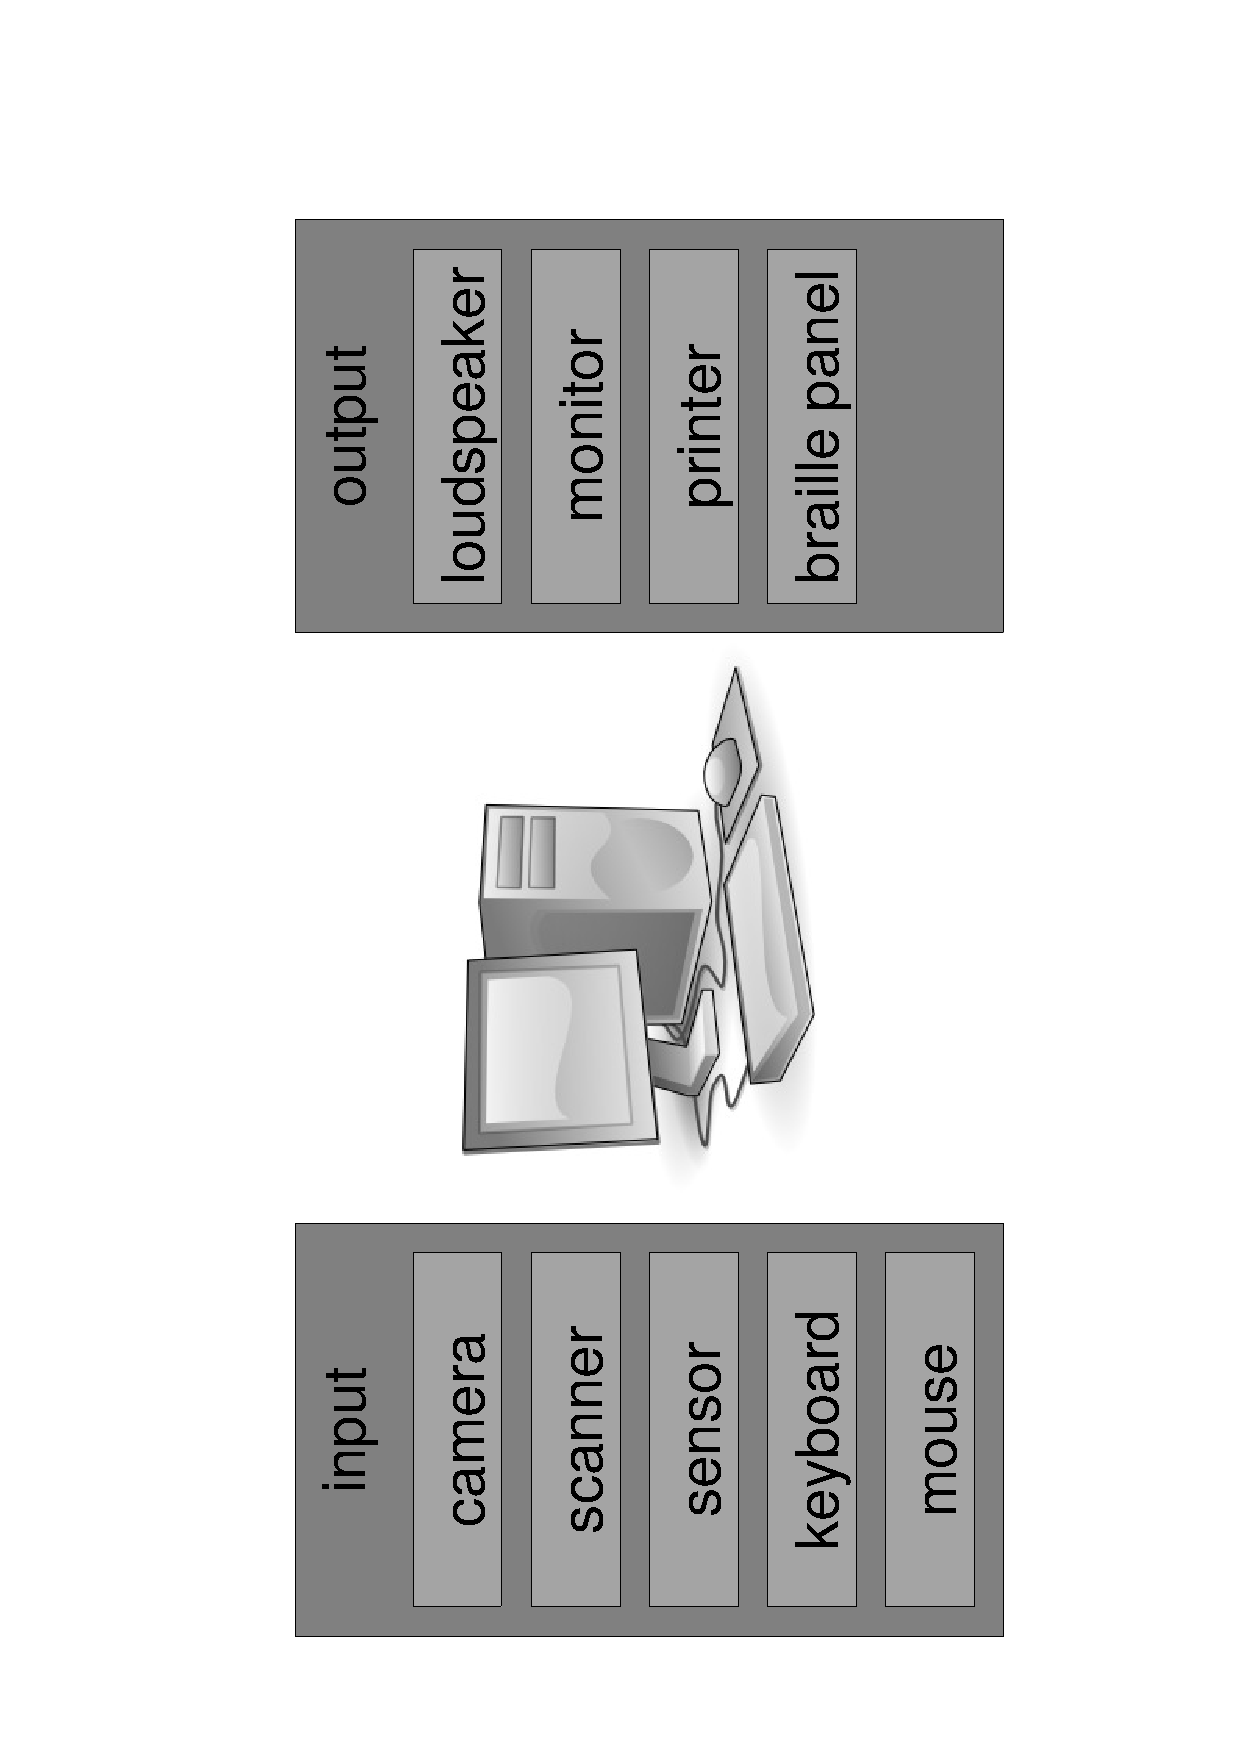
\includegraphics[scale=0.3,angle=-90]{graphic/computer.pdf}
        \caption{Computer Hardware with Input- and Output Devices}
        \label{computer_figure}
    \end{center}
\end{figure}

The difference to \emph{Robotics} is that a robot has additional devices.
Various \emph{Sensors} are used for information input; many moveable parts like
\emph{Arms} or \emph{Wheels} take motoric action and can be compared to the
extremities of the human body. Table \ref{environment_table} gives an
impression of how technical and biological environments can be compared.

\begin{figure}[ht]
    \begin{center}
        \begin{footnotesize}
        \begin{tabular}{| p{25mm} | p{50mm} | p{30mm} |}
            \hline
            \textbf{Ontological Level} & \textbf{Technical System} & \textbf{Biological Equivalent}\\
            \hline
            Network & Internet, Wide Area Network (WAN) & Society, Biotope\\
            \hline
            Family & Local Area Network (LAN) & Family\\
            \hline
            System & Computer & Organism\\
            \hline
            Block & Component & Organ\\
            \hline
        \end{tabular}
        \end{footnotesize}
        \caption{Ontology comparing Technical- and Biological Environment}
        \label{environment_table}
    \end{center}
\end{figure}

To sum up: Among the abstract knowledge models stored in a system are some that
describe the structure and capabilities of the system itself.

